\documentclass{standalone}
\usepackage{tikz}
\begin{document}

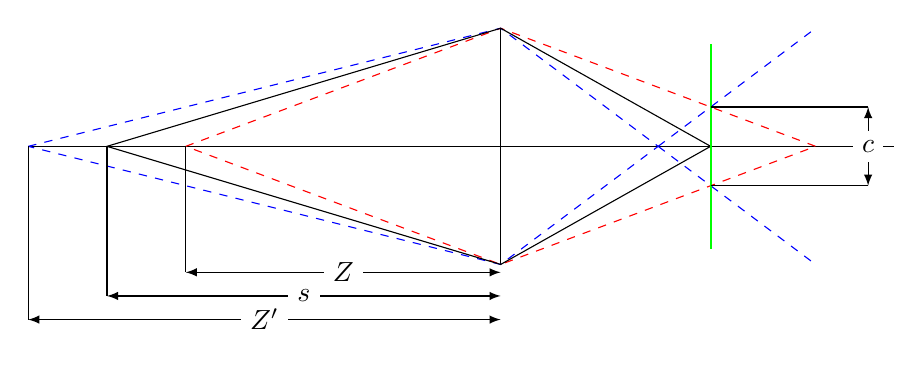
\begin{tikzpicture}

%\namedhorline{text}{textpos}{radius}
\newcommand*{\namedhorline}[3]{%
	%\draw [<-] ++ -- ++(\dx,\dy) -- ++(\dx,-\dy) -- ++(-\dx,-\dy) -- cycle
	\draw [->] (#2) +(-0.2,0) -- +(-#3,0);
	\node at (#2) {#1};
	\draw [->] (#2) +(0.2,0) -- +(#3,0);
}

%\namedhorline{text}{textpos}{radius}
\newcommand*{\namedhorlinetwo}[3]{%
	%\draw [<-] ++ -- ++(\dx,\dy) -- ++(\dx,-\dy) -- ++(-\dx,-\dy) -- cycle
	\draw [->] (#2) +(-0.2,0) -- +(-#3,0);
	\node at (#2) {#1};
	\draw [->] (#2) +(0.2,0) -- +(#3,0);
}

% http://tex.stackexchange.com/questions/14901/dimensioning-of-a-technical-drawing-in-tikz
\tikzset{%
    dimen/.style={<->,>=latex,thin,every rectangle node/.style={fill=white,midway,font=\sffamily}},
}


\def\hei{1.5}
\def\sensor{1.3}

\def\Opx{-4}
\def\Oppx{-6}
\def\Ox{-5}
\def\Ipx{4}
\def\Ippx{2}
\def\IxX{2/(1/\Ipx+1/\Ippx)}
\def\Ix{{\IxX}}
% circle of confusion radius
\def\coc{{\hei*(1-\IxX/\Ippx}}

\def\flabely{2}
\def\alabely{3}

% background and lens
\draw [thin] (\Ox-1, 0) -- (\Ipx+1, 0);
\draw [thin] (0,-\hei) -- (0, \hei);

% diamonds
\draw [dashed,red] (\Opx, 0) -- (0, \hei) -- (\Ipx, 0) -- (0, -\hei) -- cycle;

\draw [dashed,blue] (\Oppx, 0) -- (0, \hei) -- (\Ippx, 0) -- (0, -\hei) -- cycle;
\draw [dashed,blue] (\Ippx, 0) -- (2*\Ippx, -\hei);
\draw [dashed,blue] (\Ippx, 0) -- (2*\Ippx, \hei);

\draw (\Ox, 0) -- (0, \hei) -- (\Ix, 0) -- (0, -\hei) -- cycle;

\draw [thick, green] (\Ix, -\sensor) -- (\Ix, \sensor);
\draw (\Ix, \coc) -- ++(2, 0) coordinate (S1b);
\draw (\Ix, -\coc) -- ++(2, 0) coordinate (S2b);
\draw [dimen] (S1b) -- (S2b) node {$c$};

% distance arrows
\draw (\Opx, 0) -- ++(0, -\hei-0.1) coordinate (D);
\draw [dimen] (D) -- ++(-\Opx,0) node {$Z$};
\draw (\Ox, 0) -- ++(0, -\hei-0.4) coordinate (D);
\draw [dimen] (D) -- ++(-\Ox,0) node {$s$};
\draw (\Oppx, 0) -- ++(0, -\hei-0.7) coordinate (D);
\draw [dimen] (D) -- ++(-\Oppx,0) node {$Z'$};

\end{tikzpicture}

\end{document}
